\documentclass[../main.tex]{subfiles}

\begin{document}
	\section{Light}
	\begin{preamb}
		Light can be studied as a wave. In this chapter we will look at how light interacts with matter.
	\end{preamb}

	\subsection{Reflection}
	\pdef{Normal}{The normal is an imaginary line draw perpendicular to the surface that reflection is taking place at.}

	\pdef{Angle of Incidence}{The angle of incidence is the angle between the incident ray and the normal.}

	\pdef{Angle of Reflection}{The angle of reflection is the angle between the reflected ray and the normal.}

	\begin{center}
		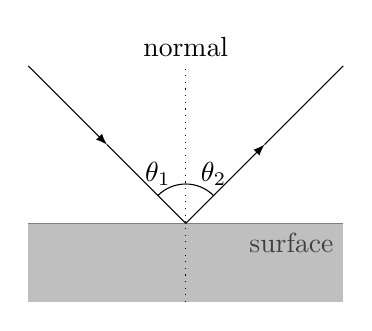
\begin{tikzpicture}
			\draw [color=gray] (-2,0) -- (2,0);
			\node [anchor=north east] at (2,0) {surface};
			\fill [color=gray, fill opacity=0.5] (-2,-1) -- (-2,0) -- (2,0) -- (2, -1);
			\draw [dotted] (0,-1) -- (0,2) node [anchor=south] {normal};
			\draw [-latex] (-2,2) -- (-1,1);
			\draw (-1,1) -- (0,0);
			\draw (0,0.5) arc (90:135:0.5) node [anchor=south] {\(\theta_1\)};
			\draw (0,0.5) arc (90:45:0.5) node [anchor=south] {\(\theta_2\)};
			\draw [-latex] (0,0) -- (1,1);
			\draw (1,1) -- (2,2);
		\end{tikzpicture}
	\end{center}

	\pdef{First Law of Reflection}{The incident ray, reflected ray, and the normal lie on the same plane.}

	\pdef{Second Law of Reflection}{In reflection, the angle of incidence is equal to the angle of reflection. \[\theta_1 = \theta_2\]}
	
	I have chosen to name the angles \(\theta_1\) and \(\theta_2\) due to the reversible nature of light. It does not matter which way the light goes; the angles will be preserved.
	
	\pdef{Virtual Image}{A virtual image is an image that cannot be cast on a screen.}
	
	The properties of an reflected image are:
	\begin{itemize}
		\item same shape and size
		\item same distance from the mirror
		\item laterally inverted
		\item upright
		\item virtual
	\end{itemize}
	
	\begin{center}
		\begin{tikzpicture}
			\draw (0,2.25) -- (0,-3);
			\fill [pattern=north east lines] (0,-3) node[anchor=north] {mirror} rectangle (0.1,2.25);
			\draw [line width=0.5mm, -latex] (-2,-1) -- (-3,1) node[anchor=east, pos=0.5] {object};
			\draw [dashed, line width=0.5mm, -latex] (2,-1) -- (3,1) node[anchor=west, pos=0.5] {image};
			\draw [dashed, color=gray] (-2,-1) -- (2,-1);
			\draw [dashed, color=gray] (-3,1) -- (3,1);
			\fill (-2,-2.5) circle (0.05) node[anchor=north] {observer};
			\draw [-latex] (-2,-1) -- (0,-1.75) node (a) {};
			\draw [-latex] (-3,1) -- (0,-1.125) node (b) {};
			\draw [latex-] (-2,-2.5) -- (a);
			\draw [latex-] (-2,-2.5) -- (b);
			\draw [dashed, -latex] (2,-1) -- (a);
			\draw [dashed, -latex] (3,1) -- (b);
		\end{tikzpicture}
		\begin{framed}
			Virtual images or construction lines are drawn with \textbf{dotted} lines.
		\end{framed}
	\end{center}
	
	\subsection{Refraction}

	\pdef{Refraction}{Refraction is the bending of light as light passes from one optical medium to another, due to light changing speed.}

	\subsubsection{Essentials}

	\pdef{Angle of Refraction}{The angle of refraction is the angle between the refracted ray and the normal.}

	\begin{center}
		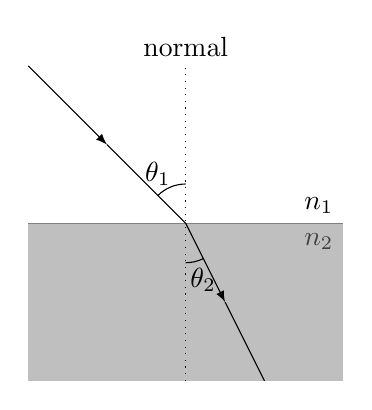
\begin{tikzpicture}
			\node [anchor=south east] at (2,0) {\(n_1\)};
			\node [anchor=north east] at (2,0) {\(n_2\)};
			\draw [color=gray] (-2,0) -- (2,0);
			\fill [color=gray, fill opacity=0.5] (-2,-2) -- (-2,0) -- (2,0) -- (2,-2);
			\draw [dotted] (0,-2) -- (0,2) node [anchor=south] {normal};
			\draw [-latex] (-2,2) -- (-1,1);
			\draw (-1,1) -- (0,0);
			\draw (0,0.5) arc (90:135:0.5) node [anchor=south] {\(\theta_1\)};
			\draw (0,-0.5) arc (270:296:0.5) node [anchor=north] {\(\theta_2\)};
			\draw [-latex] (0,0) -- (0.5,-1);
			\draw (0.5,-1) -- (1,-2);
		\end{tikzpicture}
	\end{center}

	\pdef{First Law of Refraction}{The incident ray, refracted ray, and the normal lie on the same plane.}

	\pdef{Second Law of Refraction}{For two given media, the ratio of the sine of the angle of incidence to the sine of the angle of refraction is a constant.}

	\peqn{Refractive Index}{The refractive index of a medium is the ratio of the speed of light in vacuum to the speed of light in the medium}{n = \frac{c}{v}}
	Sometimes it might also be \[ n = \frac{\text{real depth}}{\text{apparent depth}}\].

	\peqn{Snell's Law}{Snell's Law is the same thing as the second law of refraction, mathematically expressed as}{n_1 \sin \theta_1 = n_2 \sin \theta_2}

	\pdef{Critical Angle}{The critical angle is defined as the angle of incidence in an optically denser medium for which the angle of refraction in the optically less dense medium is \SI{90}{\degree}.}

	Derivation for critical angle formula for any refractive indices considering \(n_1 > n_2\), from equation 13.2,
	\begin{align*}
        n_1 \sin \theta_c &= n_2 \sin \SI{90}{\degree} \\
        \sin \theta_c &= \frac{n_2 (1)}{n_1} \\
        \sin \theta_c &= \frac{n_2}{n_1} \\
        \theta_c &= \boxed{\sin^{-1} \left(\frac{n_2}{n_1}\right)}
    \end{align*}

	\pdef{Total Internal Reflection}{Total internal reflection is the complete reflection of a light ray inside an optically denser medium at its boundary with an optically less dense medium.}

	\begin{center}
		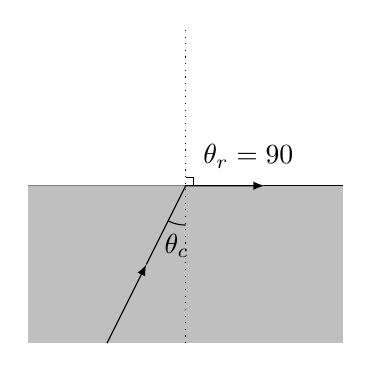
\begin{tikzpicture}
			\draw [color=gray] (-2,0) -- (2,0);
			\fill [color=gray, fill opacity=0.5] (-2,-2) rectangle (2,0);
			\draw [dotted] (0,-2) -- (0,2);
			\draw [-latex] (-1,-2) -- (-0.5,-1);
			\draw [-latex] (-0.5,-1) -- (0,0) -- (1,0);
			\draw (1,0) -- (2,0);
			\draw (0,-0.5) arc (270:244:0.5) node [anchor=north, pos=0.5] {\(\theta_c\)};
			\draw (0,0.1) -- (0.1,0.1) node [anchor=south west] {\(\theta_r = \SI{90}{\degree}\)} -- (0.1,0);
		\end{tikzpicture}
	\end{center}

	\subsubsection{Lenses}
	
	For the most part of this section, we will consider a thin lens.
	
	\begin{center}
		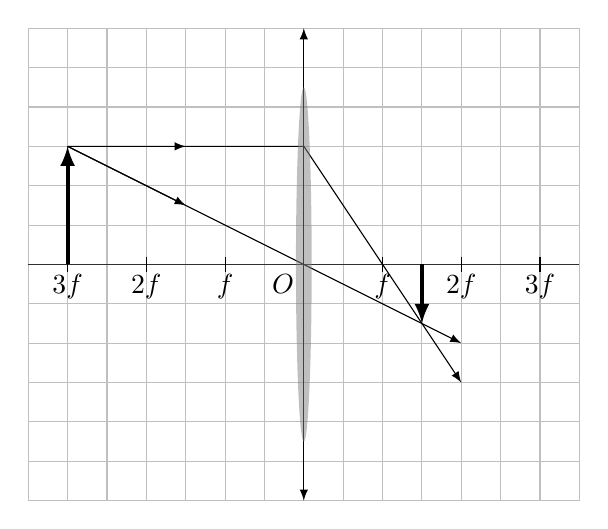
\begin{tikzpicture}
			\draw [black, opacity=0.25, step=0.5] (-3.5,-3) grid (3.5,3);
			\draw [color=black, opacity = 0.75] (-3.5,0) -- (3.5,0);
			\draw [latex-latex] (0,-3) -- (0,3) node[anchor=north east, pos=0.5] {\(O\)};
			\node [anchor=north] at (-1,0) {\(f\)}; 
			\node [anchor=north] at (1,0) {\(f\)}; 
			\node [anchor=north] at (-2,0) {\(2f\)}; 
			\node [anchor=north] at (2,0) {\(2f\)}; 
			\node [anchor=north] at (-3,0) {\(3f\)}; 
			\node [anchor=north] at (3,0) {\(3f\)}; 
			\foreach \x in {-3, -2, -1, 1, 2, 3} \draw (\x, 0.1) -- (\x, -0.1);
			\draw [-latex] (-3, 1.5) -- (0,1.5) -- (1,0) -- (2,-1.5);
			\draw [-latex] (-3, 1.5) -- (0,0) -- (2, -1);
			\draw [-latex] (-3, 1.5) -- (-1.5,1.5);
			\draw [-latex] (-3, 1.5) -- (-1.5,0.75);
			\draw [line width=0.5mm, -latex] (1.5,0) -- (1.5,-0.75);
			\draw [line width=0.5mm, -latex] (-3,0) -- (-3,1.5);
			\fill [gray, opacity=0.5] (0,0) ellipse (0.1 and 2.25);
		\end{tikzpicture}
		\begin{framed}
			Real images are drawn with \textbf{solid} lines.
		\end{framed}
	\end{center}
	
	\pdef{Principal Axis}{The horizontal line passing through the optical centre of the lens is called the principal axis. The principal axis is perpendicular to the vertical plane of the lens.}
	
	\pdef{Optical Centre}{The optical centre is the midpoint between the lens' surface on the principal axis. Rays that travel through the optical centre are not deviated.}
	
	\pdef{Focal Length}{The focal length is the distance between the optical centre and the focal point.}
	
	\pdef{Focal Plane}{The focal plane is the plane that passes through the focal point \(f\) and is perpendicular to the principal axis.}
	
	\begin{center}
		\begin{tabularx}{0.95\linewidth}{cccX}
			\hline \hline
			\(s\)\ & Image is & \(s'\) & Uses \\ 
			\hline 
			\(s=\infty\) & real & \(s'=f\) & telescope \\  
			\(s>2f\) & real & \(f<s'<2f\) & camera \\  
			\(s=2f\) & real & \(s'=2f\) & photocopier \\  
			\(f<s<2f\) & real & \(s'>2f\) & projector \\  
			\(s=f\) & virtual & \(s'=-\infty\) & eyepiece \\  
			\(s<f\) & virtual & \(s'<0\) & microscope \\ 
			\hline \hline
		\end{tabularx} 
	\end{center}

	Real images are inverted; virtual images are upright.
	
	\peqn{Thin Lens Equation}{(\textit{This is not in syllabus.}) For a thin lens, the focal length and the distances between the object and its image is }{\frac{1}{s} + \frac{1}{s'} = \frac{1}{f}}
	
	\peqn{Magnification}{(\textit{This is not in syllabus.}) The magnification of a lens is given by}{M = \frac{s'}{s}}
\end{document}
